% !TEX root = master.tex

\chapter{Model Order Reduction}
\label{Ch:ROM}
%\pagenumbering{arabic}


In this chapter model order reduction (MOR) of the BGK-model in the Sod shock tube will be introduced for which POD and in particular autoencoders are adopted to obtain a reduced basis (RB).\\
Model order reduction is a technique used for reducing the computational cost when evaluating PDE's \cite{Bernard}\cite{Carlberg}\cite{ohlberger2015reduced}. To achieve this, the solution to a PDE is being approximated by reducing one or more of it's dimensions. The reduction is performed by a mapping onto a low dimensional manifold. In our case the solution to the BGK-model is a function \(f(x,v,t) \in \mathbb{R}^3\). Now we could reduce i.e. \(v\) to \(n\), where \(o\) represents the number of elements in \(v\) and \(p\) represents the number of elements in \(n\). With \(p << o\) we obtain a reduced order model (ROM) which we call \(q(x,n,t)\) of significantly lower dimension. In particular \(n\) is called the reduced basis or the intrinsic variables. In \cref{Ch:BGK} we saw that the BGK-model is a PDE which through discretization in the spatial dimension \(x\) and the velocity dimension \(v\) holds a system of \(KJ\) ODE's in time in 1D and \(K^3J^3\) ODE's in time in 3D.  By the reduction of \(v\) we arrive at \(nJ\) ODE's in time for 1D and \(nJ^3\) ODE's in time in 3D. This example illustrates the amount of computations that can be saved by MOR. The mapping from \(f(x,v,t)\) to \(q(x,n,t)\) can be performed by one of the reduction algorithms from \cref{Ch:DimRedAl}. The remapping back to \(\tilde{f}(x,v,t)\) is carried out by the same algorithm under the condition, that the distance \(||f - \tilde{f}||\) is small.\\
To sum up, the idea that every high dimensional dynamical-state space \(W\), also called solution manifold, where in our case \(f(x,v,t) \in W\), can be mapped onto a state-space i.e. \(V\) of lower dimension with \(q(n,\mu_i) \in V\), is exploited within MOR \cite{ohlberger2015reduced}. Here \(i\) counts through the variables that where omitted during reduction and \(n\) beeing the intrinsic variables. Again \(p\) counts through the intrinsic variables. The state space of lower dimension is called the intrinsic solution manifold \(V\) with \(q(n,\mu_i) \in V\) \cite{Carlberg}.\\
\begin{figure}[H]
	\begin{subfigure}{.45\textwidth}
		\centering
		\tikzstyle{reco} = [rectangle,minimum height=4em,text centered, fill=blue!20,draw=black]
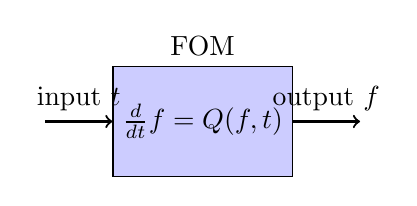
\begin{tikzpicture}[scale=0.5]
	\node [reco,label=FOM] (phys) {$\frac{d}{dt}f = Q(f,t)$};
	\draw [<-,thick] (phys)--+ (-4,0) node[midway,above] {input \(t\)};
	\draw [->,thick] (phys)--+ (4,0) node[midway,above] {output $f$};
\end{tikzpicture}

		\subcaption{Evolving the BGK-model in the Sod shock tube in time is generated through evaluating the FOM in space \(x\), velocity \(v\) and time \(t\), which yields the solution \(f(x,v,t)\). The operator \(Q\) is here the FOM described in \cref{Ch:BGK}.}
	\end{subfigure}\hfill
	\begin{subfigure}{.45\textwidth}
		\centering
		\tikzstyle{reco} = [rectangle,minimum height=4em,text centered, fill=blue!20,draw=black]
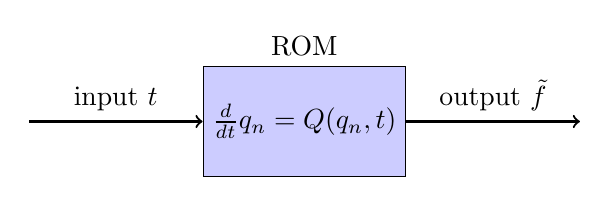
\begin{tikzpicture}[auto]
	\node [reco,label=ROM] (red) {$\frac{d}{dt}q_n = Q(q_n,t)$};
	\draw [<-,thick] (red)--+ (-3.5,0) node[midway,above] {input \(t\)};
	\draw [->,thick] (red)--+ (3.5,0) node[midway,above] {output $\tilde{f}$};
\end{tikzpicture}

		\subcaption{Evolving the ROM of the BGK-model in the Sod shock tube in time through evaluating the ROM at \(n\) and \(\mu_i\), yields an approximation to the FOM solution \(\tilde{f}\). The operator \(Q\) is here either POD or a autoencoder described in \cref{Ch:DimRedAl}.}
	\end{subfigure}
	\caption{Outline of the correlation between the FOM solution and the approximation obtained from the ROM.}
\end{figure}
MOR is partitioned into two successive phases called the \textit{offline} - and the \textit{online} phase. During the offline phase \textit{snapshots} of a dynamical-system are generated through experiments or simulations of the full order model (FOM). The snapshots \(F = \{f(t_1),...,f(t_n)\}\) are created once, each representing one moment in time of the dynamical system. Thus in our case one needs a snapshot database of solutions \(f(x,v,t)\) of the BKG-model in the Sod shock tube. Next a mapping \(Q\) is constructed such that \(\tilde{f} = Q(f)\), for which \(f(t_i) \approx \tilde{f}(t_i)\), reducing the dimensionality of the FOM solution as outlined before. During the online phase the reduced order model is evaluated and the error is estimated by 
\begin{equation}
	\L2 = \frac{||f - \tilde{f} ||_2}{||f||_2}
\end{equation}
which is called the relative \(\L2\)-Error norm. The abbreviation \(\L2\)-Error is used from here on. Therefore the online phase may be described as a stage of independence from the full order model.
Following \cite{ohlberger2015reduced} and \cite{Carlberg}, the success when building a ROM through linear reduction methods like the POD \cref{Sec: POD}, depends on a rapidly decaying Kolmogorov N-width. In particular advection dominated problems exhibit a slow decay of the Kolmogorov N-width. Thus yielding a need for non-linear methods like autoencoders described in \cref{Sec:AE}. The Kolmogorov N-width is given by
\begin{equation}
	d_{V}(W):= \sup_{f \in W} \inf_{\tilde{f} \in V} ||f-\tilde{f}||
	\label{Eq:Kolmogorov}
\end{equation}
and gives the worst best approximation error for elements of \(W\). The convergence behaviour of the Kolmogorov N-width for advection dominated problems, especially when jump conditions are involved as in the Sod shock tube \cref{Ch:BGK}, decays with
\begin{equation}
	d_n(W) \leq \frac{1}{2} n^{-1/2},
	\label{Eq:KolmoAdv}
\end{equation}
where \(n\) denotes the number of RB or intrinsic variables. Note that hereafter we will solely use the term intrinsic variables\cite{ohlberger2015reduced}. The relevance of using non-linear reduction methods for MOR is often formulated in terms of a slow decaying Kolmogorov N-width. Altough BGK-model in the sod shock tube describes an advection problem with jump discontinuities \cref{Ch:BGK} implies that linear reduction methods should fail. But we will see in the following that this is only partly true for this study.
\section{Offline Phase}
\subsection{Full order BGK-model}\label{Sec: FOM}
The FOM is the 1D BGK-model in the Sod shock tube for two levels of rarefaction, gratefully provided by Julian K\"ollermeier and the Departement of Mathematics at the RWTH Aachen. The Sod shock tube is discretized in space \(x\) with 100 nodes, in velocity \(v\) with 40 nodes for 25 time steps in time \(t\), as presented in \cref{Tab:Setup} and \cref{Fig:SodProbSetup}. Details about the BGK-model and Sod's shock can be found in \cref{Ch:BGK}.
\begin{table}[htp]
	\centering
	\caption{Problem setup for the BGK model in the Sod shock tube. The diaphragm is positioned at \(x_d=0.5025\). For \(x<x_d\) the gas is present, for \(x\geq x_d\) particles are absent.}
	\begin{tabular*}{15cm}{ @{\extracolsep{\fill}} c c c c @{} }
		\toprule
		Variable   & Number of nodes \(i\)&   Domain extension& Step size (uniform)\\   
		\hline
		\(x\) 		&	200&     [0.0025,0.9975]&	    0.00499\\
		\(v\)       &   40 &  		    [-10,10]&	    0.05128\\
		\(t\)   	&	25 &        	[0,0.12]&	      0.005\\
		\bottomrule
	\end{tabular*} \label{Tab:Setup}
\end{table}
One can be viewed as a slip flow \cite{schaaf} with \(\Kn=0.01\), hereafter referred to as \(\rare\). The dilution up to this level of rarefaction is little though leading to inaccuracies when employing the common Navier Stokes equations. Therefore the NFS-equations (Navier-Stokes-Fourrier) could be used \cite{NumaKUL}. The other is situated in the continuum flow regime with \(\Kn=0.00001\) for which the Navier-Stokes equations can be utilized without hesitation. A detailed description can be found in \cref{Ch:BGK}. Hereafter the continuum flow will be referred to as \(\hy\). Note that both \(\hy\) and \(\rare\) are three dimensional tensors containing \(f(x,v,t)\).\\
The reduction algorithms, introduced in \cref{Ch:DimRedAl}, require a distinct reshaping of the input data before they can be used. The preprocessed matrix for the FCNN, \(\mae\), is shown in \cref{Eq:AE_matrix}. Each row of \(\mae\) contains a sample shown to the FCNN. In turn we aquire \(x_it_i=5000\) samples. The preprocessed matrix for the CNN, \(\mconv\), is shown in \cref{Eq:CNN_matrix}. We obtain \(v_i=40\) samples, each containing a matrix \(\pi_{CNN}^{x_i\times t_i}\) holding the information about \(f(x,t)\) for a fixed point in \(v\). POD uses the \(\mae\) matrix or its transposition.\\
\begin{minipage}{.55\linewidth}
	\begin{equation}
	\mae = \begin{bmatrix}
	f(v_1,t_1,x_1)&\cdots &f(v_n,t_1,x_1) \\
	f(v_1,t_1,x_2)&\cdots &f(v_n,t_1,x_2) \\
	\vdots& \vdots & \vdots\\
	f(v_1,t_1,x_n)&\cdots &f(v_n,t_1,x_n)\\
	f(v_1,t_2,x_1)&\cdots &f(v_n,t_2,x_1)\\
	\vdots & \vdots & \vdots\\
	f(v_1,t_n,x_n)&\cdots &f(v_n,t_n,x_n)
	\end{bmatrix}
	\label{Eq:AE_matrix}
	\end{equation}
\end{minipage}%
\begin{minipage}{.45\linewidth}
	\begin{equation}
	\mconv= \begin{bmatrix}
	n_{Filters},&f(v_1,\textbf{t},\textbf{x})\\
	n_{Filters},&f(v_2,\textbf{t},\textbf{x})\\
	\vdots&\vdots\\
	n_{Filters},&f(v_n,\textbf{t},\textbf{x})
	\end{bmatrix}
	\label{Eq:CNN_matrix}
	\end{equation}
\end{minipage}\\\\
In the following a distinction between \(\mconv\) and \(\mae\) is omitted, when referring to the preprocessed matrices. However a distinction between the levels of rarefaction, namely \(\hy\) and \(\rare\), will be utilized as \(\mhy\) for the former and \(\mrare\) for the latter. This designation is mainly used in \cref{Ch:ApB} and \cref{Ch:ApA}.
\subsection{Contructing the mapping}
With the FOM solution at hand it is possible to construct a mapping \(Q\) such that \(Q(f)\approx \tilde{f}\). For \(Q\), POD and two autoencoders, based on a fully connected neural network (FCNN) and a convolutional neural network (CNN), are employed, see \cref{Ch:DimRedAl}. The selection of hyperparameters and training for the FCNN and the CNN is discussed in \cref{Ch:ApA} and \cref{Ch:ApB}. Hence the availability of fully trained and tuned FCNN and CNN is given from now on. Since this thesis focuses on the use of neural networks, POD acts as a benchmark.\\
To continue, the intrinsic variables obtained from POD, the FCNN and the CNN, will be referred as \(\idhy\) and \(\idrare\). The former describes the intrinsic variables when reducing \(\hy\) and the latter when reducing \(\rare\).\\
In order to contrast the number \(p\) of intrinsic variables in the autoencoders (sizes of \(\idhy\) and \(\idrare\)) we will utilize POD as a reference framework. Therefore the singular values \(\sigma\), as well as, the cumulative energy (cusum-e)\\
\noindent \begin{minipage}{.3\linewidth}
	\begin{equation}
	\textrm{cusum-e} = \frac{\textrm{cusum}}{\sum_i \sigma_i}
	\end{equation}
\end{minipage}%
\begin{minipage}{.7\linewidth}
	\begin{equation}
			\textrm{with} \qquad\qquad(\textrm{cusum})_i =(\text{cusum})_{i-1} + \sigma_{i}
	\end{equation}
\end{minipage}\\\\
over the singular values, are employed. A comparison for both levels of rarefaction is provided in \cref{Fig:CUSUM-e}. With a total of \(p=4\) intrinsic variables, a cumulative energy of over \(99\%\) can be achieved for \(\hy\). The fourth singular value measures to a value of \(\sigma_4 = 0.706\). The cumulative energy of the singular values of \(\rare\) arrives above \(99\%\) with \(p=6\) singular values. The sixth value is at \(\sigma_6 = 0.275\). The rate at which the singular values drop is exponential in \(\hy\) and in \(\rare\), with a difference of \(\L2 = 0.025\) in the \(\L2\)-Error when comparing the gradients of the first \(p=10\) singular values. This should highlight the different characteristics when being reduced between both data sets.\\
We can link the decay of the Kolmogorov N-width in \cref{Eq:Kolmogorov} with the decay of the singular values, which invalidates the application of \cref{Eq:KolmoAdv} for the FOM solution. For both \(\hy\) and \(\rare\) the singular values and in turn the Kolmogorov N-width decay rapidly, which in turn leads to the assumption that advection and sharp shock fronts do not appear predominantly. Moreover the dissimilarly decay rate is a manifestation of the differing rarefaction levels. With a decreasing number of particles present, the lesser the probability of a single bulk macroscopic velocity emerges, see a full survey in \cref{Ch:BGK}. Therefore \(\idhy\) can always be chosen smaller than \(\idrare\), written as \(\idhy < \idrare\), which is also evident with the FCNN and the CNN as discussed in the following.   
\begin{figure}[H]
	\begin{subfigure}{.45\textwidth}
		% This file was created by tikzplotlib v0.9.6.
\begin{tikzpicture}

\begin{groupplot}[group style={group size=2 by 1, horizontal sep=1cm, vertical sep=2cm}]
\nextgroupplot[
log basis y={10},
tick align=outside,
tick pos=left,
x grid style={white!69.0196078431373!black},
xlabel={\(k\)},
xmin=-0.95, xmax=41.95,,
xtick style={color=black},
y grid style={white!69.0196078431373!black},
ylabel={\(\sigma\)},
ymin=2.86160392849359e-16, ymax=240.32740800328,
ymode=log,
ytick style={color=black},
ytick={1e1,1e-3,1e-11,1e-15},
width=.55\textwidth,
height=.7\textwidth,
y label style={yshift=-2.5em},
grid=both
]
\addplot [semithick, red, mark=o, mark size=2, mark options={solid}]
table {%
1 36.8185958349281
2 5.78483852846218
3 2.9488881352441
4 1.08115123432794
5 0.4715894924307
6 0.27551553286601
7 0.155493855631619
8 0.0601331453526982
9 0.05155511017701
10 0.0132542951500055
11 0.0118122790965581
12 0.00208495452053553
13 0.00184461993287337
14 0.000261109297076443
15 0.000174118703867616
16 2.59262125849959e-05
17 1.30752219185821e-05
18 1.92140998809572e-06
19 9.1685066176197e-07
20 1.08651788755093e-07
21 5.26354986735524e-08
22 4.52124036969183e-09
23 2.44729256168519e-09
24 1.43747068296607e-10
25 9.28350136149776e-11
26 3.39879764456285e-12
27 2.74182349854538e-12
28 6.4789443879917e-14
29 6.12293316992491e-14
30 1.6313694307166e-14
31 2.92181471455653e-15
32 2.92181471455653e-15
33 2.92181471455653e-15
34 2.92181471455653e-15
35 2.92181471455653e-15
36 2.92181471455653e-15
37 2.92181471455653e-15
38 2.92181471455653e-15
39 2.92181471455653e-15
40 1.8678655154319e-15
};

\nextgroupplot[
tick align=outside,
tick pos=left,
x grid style={white!69.0196078431373!black},
xlabel={\(k\)},
xmin=-0.95, xmax=41.95,
xtick style={color=black},
y grid style={white!69.0196078431373!black},
ylabel={cusum-e},
ymin=0.760859233580134, ymax=1.0113876555438,
ytick style={color=black},
ytick={1,.8},
width=.55\textwidth,
height=.7\textwidth,
y label style={yshift=-2em},
grid=both
]
\addplot [semithick, red, mark=o, mark size=2, mark options={solid}]
table {%
1 0.772246889123937
2 0.893580238655189
3 0.95543131247198
4 0.978107779579132
5 0.987999072557982
6 0.993777837563443
7 0.997039223381299
8 0.998300478281949
9 0.999381814290284
10 0.999659814794242
11 0.999907569918492
12 0.999951300528145
13 0.99998999027099
14 0.999995466874262
15 0.999999118904556
16 0.999999662690558
17 0.999999936935114
18 0.99999997723548
19 0.999999996465846
20 0.999999998744749
21 0.999999999848745
22 0.999999999943575
23 0.999999999994906
24 0.999999999997921
25 0.999999999999868
26 0.999999999999939
27 0.999999999999997
28 0.999999999999998
29 0.999999999999999
30 1
31 1
32 1
33 1
34 1
35 1
36 1
37 1
38 1
39 1
40 1
};
\addplot [thick, , mark=x,black, mark size=2, mark options={solid}]
table{%
6 0
6 0.993777837563443
6 1.3
};
\end{groupplot}
\end{tikzpicture}


		\subcaption{Sigular values \(\sigma\) over \(k\) number of singular values (left) and cumulative energy, here labeled as \glqq cusum-e\grqq{} over \(k\) (right) for \(\hy\). A black cross marker corresponds to over 99\% cumulative energy.}
		\label{Fig:CumSum_Rare}
	\end{subfigure}\hfill
	\begin{subfigure}{.45\textwidth}
		% This file was created by tikzplotlib v0.9.6.
\begin{tikzpicture}

\begin{groupplot}[group style={group size=2 by 1, horizontal sep=1cm, vertical sep=2cm}]
\nextgroupplot[
log basis y={10},
tick align=outside,
tick pos=left,
x grid style={white!69.0196078431373!black},
xlabel={\(k\)},
xmin=-0.95, xmax=41.95,,
xtick style={color=black},
y grid style={white!69.0196078431373!black},
ylabel={\(\sigma\)},
ymin=2.86160392849359e-16, ymax=240.32740800328,
ymode=log,
ytick style={color=black},
ytick={1e1,1e-3,1e-11,1e-15},
width=.55\textwidth,
height=.7\textwidth,
y label style={yshift=-2.5em},
grid=both
]
\addplot [semithick, red, mark=o, mark size=2, mark options={solid}]
table {%
1 36.8185958349281
2 5.78483852846218
3 2.9488881352441
4 1.08115123432794
5 0.4715894924307
6 0.27551553286601
7 0.155493855631619
8 0.0601331453526982
9 0.05155511017701
10 0.0132542951500055
11 0.0118122790965581
12 0.00208495452053553
13 0.00184461993287337
14 0.000261109297076443
15 0.000174118703867616
16 2.59262125849959e-05
17 1.30752219185821e-05
18 1.92140998809572e-06
19 9.1685066176197e-07
20 1.08651788755093e-07
21 5.26354986735524e-08
22 4.52124036969183e-09
23 2.44729256168519e-09
24 1.43747068296607e-10
25 9.28350136149776e-11
26 3.39879764456285e-12
27 2.74182349854538e-12
28 6.4789443879917e-14
29 6.12293316992491e-14
30 1.6313694307166e-14
31 2.92181471455653e-15
32 2.92181471455653e-15
33 2.92181471455653e-15
34 2.92181471455653e-15
35 2.92181471455653e-15
36 2.92181471455653e-15
37 2.92181471455653e-15
38 2.92181471455653e-15
39 2.92181471455653e-15
40 1.8678655154319e-15
};

\nextgroupplot[
tick align=outside,
tick pos=left,
x grid style={white!69.0196078431373!black},
xlabel={\(k\)},
xmin=-0.95, xmax=41.95,
xtick style={color=black},
y grid style={white!69.0196078431373!black},
ylabel={cusum-e},
ymin=0.760859233580134, ymax=1.0113876555438,
ytick style={color=black},
ytick={1,.8},
width=.55\textwidth,
height=.7\textwidth,
y label style={yshift=-2em},
grid=both
]
\addplot [semithick, red, mark=o, mark size=2, mark options={solid}]
table {%
1 0.772246889123937
2 0.893580238655189
3 0.95543131247198
4 0.978107779579132
5 0.987999072557982
6 0.993777837563443
7 0.997039223381299
8 0.998300478281949
9 0.999381814290284
10 0.999659814794242
11 0.999907569918492
12 0.999951300528145
13 0.99998999027099
14 0.999995466874262
15 0.999999118904556
16 0.999999662690558
17 0.999999936935114
18 0.99999997723548
19 0.999999996465846
20 0.999999998744749
21 0.999999999848745
22 0.999999999943575
23 0.999999999994906
24 0.999999999997921
25 0.999999999999868
26 0.999999999999939
27 0.999999999999997
28 0.999999999999998
29 0.999999999999999
30 1
31 1
32 1
33 1
34 1
35 1
36 1
37 1
38 1
39 1
40 1
};
\addplot [thick, , mark=x,black, mark size=2, mark options={solid}]
table{%
6 0
6 0.993777837563443
6 1.3
};
\end{groupplot}
\end{tikzpicture}


		\subcaption{Sigular values \(\sigma\) over \(k\) number of singular values (left) and cumulative energy, here labeled as \glqq cusum-e\grqq{} over \(k\) (right) for \(\rare\).  A black cross marker corresponds to over 99\% cumulative energy.}
		\label{Fig:CumSum_Hydro}
	\end{subfigure}
	\caption{Comparison of singular variables \(\sigma\) and cumulative energy for \(\hy\) and \(\rare\). The decay of the singular values can be used to estimate the decay of the Kolmogorov n-width.}
	\label{Fig:CUSUM-e}
\end{figure}
From a fluid mechanical point of view the number of intrinsic variables for \(\hy\) should be in total not more than three, as a slip-flow can be described in terms of three macroscopic quantities like density \(\rho\), macroscopic velocity \(u\) and total energy \(E_{tot}\)\cite{BGK}\cite{Bernard}. Therefore \(p=3\) is employed for \(\idhy\) and the autoencoders are arranged in that way. When considering \(\rare\) the picture becomes a little blurrier, as outlined before. More than one Maxwellian describe the microscopic velocities which increases \(p\). To shed light into the size we want to choose for \(\idrare\), the size of the bottleneck layer of the autoencoders, which is the same as \(p\) is varied in a next step.\\
To this end $p$ is varied for POD, FCNN and CNN over $p \in \{1,2,4,8,16,32\}$ with both $\hy$ and $\rare$. Note that the neural networks needed to be trained for these experiments and that by changing $p$ i.e. widening the bottleneck layer, a gain or loss of capacity occurs which can be connected to stability during training, see \cref{Ch:DimRedAl} and \cite{Goodfellow}.
\begin{figure}[htbp!]
	% This file was created by tikzplotlib v0.9.6.
\begin{tikzpicture}
\definecolor{color0}{rgb}{0.12156862745098,0.466666666666667,0.705882352941177}

\begin{groupplot}[group style={group size=2 by 1,horizontal sep=2cm}]
\nextgroupplot[
legend cell align={left},
legend style={draw=none,at={(0.03,0.03)}, anchor=south west},
log basis y={10},
tick align=outside,
tick pos=left,
x grid style={white!69.0196078431373!black},
xmajorgrids,
xmin=-0.55, xmax=33.55,
xminorgrids,
xtick style={color=black},
y grid style={white!69.0196078431373!black},
ymajorgrids,
ymin=4.38349387313967e-16, ymax=1.61134858880557,
yminorgrids,
ymode=log,
ytick style={color=black},
ytick={1e-1,1e-2,1e-3,1e-4,1e-6,1e-8,1e-10,1e-12,1e-14},
xlabel={Number of intrinsic varibales},
ylabel={\(L_2\)-Error},
width=0.47\textwidth,
height =.45\textwidth,
clip=false,
y label style={yshift=-.7em},
max space between ticks=20
]
\addplot [thick, red, mark=o, mark size=2, mark options={solid}, dashed]
table {%
1 0.188112310801957
2 0.0750338979596223
3 0.020528730333796635
4 0.00808627149114823
8 0.000193252431896578
16 3.06183124046159e-08
32 2.23530701528268e-15
};
\addlegendentry{POD}
\addplot [thick, color0, mark=pentagon, mark size=2, mark options={solid}, only marks]
table {%
1 0.00663323979824781
2 0.00234045716933906
3 0.0008
4 0.000691965571604669
8 0.000261269917245954
16 0.000194361884496175
32 0.000206562195671722
};
\addlegendentry{FCNN}
\addplot [thick, green!50!black, mark=triangle, mark size=2, mark options={solid,rotate=180}, only marks]
table {%
1 0.176033899188042
2 0.0960375890135765
4 0.0284016542136669
5 0.026
8 0.0258560031652451
16 0.0232554506510496
32 0.0237289071083069
};
\addlegendentry{CNN}
\draw[thick](3,40e-17)--(3,1.5);
\draw [thick,<-] (axis cs:3,1.5)-- +(10pt,10pt) node[right] {\(p\)};
\nextgroupplot[
legend cell align={left},
legend style={draw=none, at={(0.03,0.03)}, anchor=south west},
log basis y={10},
tick align=outside,
tick pos=left,
x grid style={white!69.0196078431373!black},
xmajorgrids,
xmin=-0.55, xmax=33.55,
xminorgrids,
xtick style={color=black},
y grid style={white!69.0196078431373!black},
ymajorgrids,
ymin=1.70008814466799e-15, ymax=0.821373329691319,
yminorgrids,
ymode=log,
ytick style={color=black},
ytick={1e0,1e-1,1e-2,1e-3,1e-4,1e-6,1e-8,1e-10,1e-12,1e-14},
xlabel={Number of intrinsic varibales},
ylabel={\(L_2\)-Error},
width=0.47\textwidth,
height =.45\textwidth,
clip=false,
y label style={yshift=-.7em},
max space between ticks=20
]
\addplot [thick, red, mark=o, mark size=2, mark options={solid}, dashed]
table {%
1 0.176637499442346
2 0.0853532495802733
4 0.015335605212791
5 0.008731715326052242
8 0.00145958547754045
16 3.54159334428613e-07
32 7.90549608414532e-15
};
\addlegendentry{POD}
\addplot [thick, color0, mark=pentagon, mark size=2, mark options={solid}, only marks]
table {%
1 0.58092600107193
2 0.00492882402613759
4 0.0029036
5 0.0009
8 0.00120856
16 0.000355097494320944
32 0.000395381561247632
};
\addlegendentry{FCNN}
\addplot [thick, green!50!black, mark=triangle, mark size=2, mark options={solid,rotate=180}, only marks]
table {%
1 0.160851925611496
2 0.0912962183356285
4 0.0309077128767967
5 0.026
8 0.0263328477740288
16 0.0228330623358488
32 0.022412983700633
};
\addlegendentry{CNN}
\draw[thick](5,16.5e-16)--(5,0.85);
\draw [thick,<-] (axis cs:5,0.85)-- +(10pt,10pt) node[right] {\(p\)};
\end{groupplot}

\end{tikzpicture}

	\caption{Variation of the number of intrinsic variables \(p\) over the $\L2$-Error for POD, FCNN and CNN. Results for $\hy$ are displayed on the left and for $\rare$ on the right.}
	\label{Fig:IntVar}
\end{figure}
Shown in \cref{Fig:IntVar} is the outcome of said experiments. The design for \cref{Fig:IntVar} is taken from \cite{Carlberg}. The loss of information when applying the POD goes exponentially to zero with increasing $p$ which is not suprising when consulting the \textit{Eckard-Young Theorem} provided in \cref{Eq:EckardYoung} taken from \cite{Kutz}.
The left plot of \cref{Fig:IntVar} displays the results for $\hy$ with $p=3$ the estimated size of \(\idhy\), emphasized with a black line. Here a drop in the $\L2$-Error can be observed for both neural networks until $p = 3$. Stagnation is observed for the CNN afterwards. FCNN continues to improve slighly. However the choice for $p=3$ can be confirmed.\\
Moving forward to establish the value of \(p\) for $\rare$ we look at the right plot of \cref{Fig:IntVar}. A drop in the $\L2$-Error can be observed for the FCNN with increasing $p$ until $p = 5$, which is highlighted with a black line. A continued widening of the bottleneck layer results in an slightly increased $\L2$-Error. Overfitting due to increased capacity of the model can be though of as the culprit here. Contrarily the CNN performs best with \(p = 4\) and maintains a zig zag pace progression. The discrepancy between \(p=4\) and \(p = 5\) in the CNN and FCNN is negligible. For one the FCNN performs overall better than it's convolutional counterpart, additionally shifts of missing nodes i.e. weights and biases in the bottleneck layer to the weights and biases of other layers makes this \glqq method\grqq{} fairly inaccurate. Thus we decide for \(p=5\) in \(\rare\).\\
A detailed survey of the reconstruction \(\tilde{f}\) obtained from POD, the FCNN and the CNN  using \(p\) is provided in \cref{Ch:Results}. 
\subsection{Online Phase}
In the online phase new states of the FOM solution are calculated. Moreover new states need to be evaluated. With POD one usually exploits the intrinsic variables within a Galerkin framework as in \cite{Bernard} and \cite{Carlberg} to produce new states, which won't discussed in this thesis. The same can be done with the intrinsic variables obtained from autoencoders as in \cite{Carlberg}. In this contribution new states are produced employing simple interpolation in time \(t\) of \(\idhy\) and \(\idrare\). This approach can be thought of as the ability of the autoencoder to generalize, an idea that stems from deep learning. Therefore the generalization ability of the proposed autoencoder architectures will be analyzed in \cref{Ch:Results}.   